\chapter{Design}\label{chapter:design}

The previous chapter introduced the reader to the concept of matrix profiles and their efficient computation, as well as key development concepts on the Cerebras Wafer Scale Engine. The following chapter presents the top-level architecture as a combination of a \texttt{Wrapper}, \texttt{Host Application} and an \texttt{Accelerated Kernel}. The presented design constitutes a tiled version of the algorithm described in Subsection \ref{subsection:accelerated_kernel}, allowing the problem size to be decoupled from the concrete kernel implementation. We also explore the various types of tiling solutions that could be incorporated.

\clearpage
\section{Architecture} \label{section:arch}

The presented design is based on a architecture consisting of 3 distinct components, namely the \texttt{Wrapper Application}, \texttt{Host Application} and the \texttt{Accelerated Kernel}. The \texttt{Wrapper Application} computes the tiles required for the time series and passes the tiles to the \texttt{Host Application}. The \texttt{Host Application} loads the time series and prepares the data to be broadcasted to the \textit{Fabric}. The \texttt{Accelerated Kernel} performs the actual computation described in Subsection \ref{subsection:tiled_kernel} on the WSE. A visualization of this architecture can be found in Figure \ref{fig:architecture}

\begin{figure}[h!]
    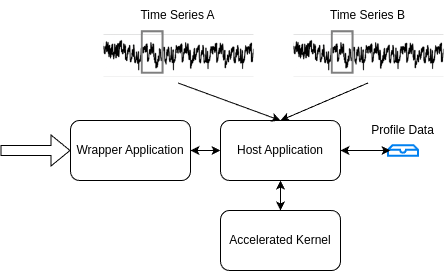
\includegraphics[scale=0.5]{architecture}
    \centering
    \caption{Architecture of our application}
    \label{fig:architecture}
\end{figure}

The computation can be divided into four distinct phases:
\begin{enumerate}
    \item \textbf{Configure Run} \texttt{Wrapper Application}: Configures the parameters for the run. Decides the \texttt{Tile Size} and \texttt{Window} and the dimensions of the \texttt{Resource Rectangle} to be allocated for execution and splits the problem space into smaller chuncks which can be executed by the \texttt{Resource Rectangle} if the available resource is not sufficient.
    \item \textbf{Pre-Computation} \texttt{Host Application}: It picks up the configuration from the \texttt{Wrapper} After the input time series are read, the statistics, i.e., $df, dg, $ and the L2-norms inverses are computed. The Host Application also computes the kernel arguments for each \texttt{Tile}. It then initializes the Simulator/Device and specifies the code to be pushed to the PEs that are part of the \texttt{Resource Rectangle}
    \item \textbf{Computation} \texttt{Accelerated Kernel}: Once the data is transfered, The Host calls the \textit{compute} function which triggers the computation on all PEs allocated in the \texttt{Resource rectangle}. After all tiles have successfully been computed by the device, The Host can read the row- and column-aggregates from the device.
    \item \textbf{Post Computation} \texttt{Host Application}: The next step in the computation is to merge the MP and MPI results from the tiles into a single Matrix Profile.
\end{enumerate}


\subsection{Accelerated Kernel} \label{subsection:accelerated_kernel}

Cerebras Software Language, or CSL, shares syntax similarities with languages like Go, Swift, and Scala. It is tailored for crafting high-performance programs for Processing Elements (PEs) on the Wafer Scale Engine (WSE). CSL operates as a medium-level language, providing access to both low and high-level programming features. At a low level, CSL exposes the functionalities of the instruction set and some hardware structures controlled by the Instruction Set Architecture (ISA). Conversely, CSL behaves as a high-level language, supporting structured control flow, loops, if-then-else constructs, and abstracting processor registers with automatic register allocation. Additionally, CSL facilitates compile-time execution of code blocks that take compile-time constant objects as input, a potent capability inherited from Zig, the language CSL is based on. Although CSL will be familiar to individuals proficient in C/C++, it incorporates new features atop the basics derived from C.

The entry point to a CSL program is through defining the \texttt{Resource Rectangle} for the given program as depicted in Figure \ref{code:distribute_kernel}. This specifies the number of PEs that needs to allocated for computation. The language also provides the flexibility to allocate specific regions of the \texttt{Resource Rectangle} for different computational requirements. For our usecase, we have a kernel implementation that is pushed into every PE that is allocated in the \texttt{Resource Rectangle}. Figure \ref{code:distribute_kernel} is an extract of code that allocates a \texttt{Resource Rectangle} of size \texttt{WIDTH}, \texttt{HEIGHT} and pushes the code \texttt{tile\_kernel.csl} to each of the PE. There is also the provision to pass params to each PE and the ability to modify them based on the requirements.

\begin{figure}[!ht]
    \centering
    \begin{minted}[mathescape, breaklines, frame=single, fontsize=\footnotesize]{text}
@set_rectangle(WIDTH, HEIGHT);
for (@range(i16, WIDTH)) | x | {
    for (@range(i16, HEIGHT)) | y | {
        @set_tile_code(x, y, "tile_kernel.csl", .{ 
            .memcpy_params = memcpy.get_params(x),
            .LEN = LEN,
            .WINDOW = WINDOW,
            .N = LEN - WINDOW + 1,
        });
    }
}
\end{minted}
\caption{Setting a \texttt{Resource Rectangle} of size \texttt{WIDTH} and \texttt{HEIGHT} and distributing \texttt{tile\_kernel.csl} to each PE with params for \texttt{Tile Size} and \texttt{window}}
\label{code:distribute_kernel}
\end{figure}

\subsection{Host Application} \label{subsection:host}

The \texttt{Host Application} provides a path to the binaries produced by the CSL compiler, prepares the data required for execution and distributes the data to the allocated PEs.
Once the kernel has finished computation on all the PEs, the host reads the profiles from the fabric and they are then reordered and reduced on the host. The Matrix Profile is then persisted onto a file.

The execution flow for the simulator and device are slightly different. The device compiler outputs an artifact id for the \texttt{SdkRuntime} to pick up and this is then executed.
The simulator on the other hand picks up the binaries compiled by the \texttt{cslc} compiler and executes them on the CPU. The SDK handles the abstractions and configures the execution on the device/simulator.

\subsection{Wrapper Application} \label{subsection:wrapper}

The Wrapper Application is a wrapper of the \texttt{Host Application} and allows flexible execution of different tile sizes ($t_s$), partial matrix profiles and different \textit{Fabric} configurations. This allowed us to test various optimizations and debug errors effectively.

\section{Kernel Algorithm} \label{section:kernel}

The following section examines the Vanilla Kernel of the Matrix Profiling algorithm, followed by an exploration of the tiled version implemented by SCAMP. Finally, it delves into the tiled version that we implemented on the Cerebras WSE-2.

\subsection{Vanilla Algorithm} \label{subsection:vanilla_kernel}

The \texttt{Vanilla Kernel} employs the update formulation described in Equation \ref{eq:qt_next_row} by iteratively computing parts of the distance matrix contained within the current diagonal chunk. Its concept is rather simple, and it provides a good foundation to explain the \texttt{Tiled Kernel} in the following subsection. Subsequently, we describe the computation performed by the Vanilla Kernel:

\begin{enumerate}
    \item Initially, the set of QT values is used to initialize the internal variables (line 1). Additionally, the local aggregate representations are initialized (lines 2 - 3). Since we are calculating Pearson correlations instead of Euclidean distances, as described in the previous section, aggregates are initialized with $-\infty$ instead of $\infty$.
    \item Subsequently, the incremental update formulation, as described in Equation \ref{eq:qt_next_row}, is employed to compute successive QT rows (line 7), and Equation \ref{eq:pearson_calculation} is used to determine the Pearson correlation (line 8). Following that, the aggregates are updated accordingly (lines 9 - 12).
    \item Once all diagonals within the current chunk have been computed, the aggregates are returned (line 15).
\end{enumerate}
    
Pseudocode for the Vanilla Kernel can be found in Algorithm \ref{alg:vanilla_kernel}.

\begin{algorithm}
\caption{Vanilla Kernel}\label{alg:vanilla_kernel}
    \hspace*{\algorithmicindent} \textbf{Input} : Time Series $T$ of length \( n \in \mathbb{N} \) and subsequence length  \( m \in \mathbb{N} \) \\
    \hspace*{\algorithmicindent} \textbf{Output} : Matrix Profile $MP$ and Matrix Profile Index $MPI$
    \begin{algorithmic}[1]
        \State $df,dg,inv \gets PreComputeStatistics(T, m);$
        \State $QT_{init} \gets PreComputeInitialQTRow(T, m);$
        \State $rowAggregates, columnAggregates \gets (-\infty, -1);$
        \For{$iteration \gets 0$ \textbf{to} $\lceil \frac{n - m + 1}{1} - 1 \rceil$}
            \State $iteration_i \gets MatrixProfileKernel(QT_{init}, $df$, $dg$, $inv$);$
            \State $UpdateAggregates(rowAggregates, columnAggregates, iteration_i);$
        \EndFor
        \State $PostCompute(rowAggregates, columnAggregates);$\\
        \Return $MP, MPI;$
    \end{algorithmic}
\end{algorithm}
    
\subsection{Tiled Algorithm} \label{subsection:tiled_kernel}

SCAMP improves on the vanilla kernel for exploiting the parallelizable nature of the problem by implementing a tiled architecture.
As explained in Equation \ref{eq:qt_next_row}, the computation of $QT_{i,j}$ requires just the time series at that point, that and the precomputed statistics, enabling every tile to be computed independently.
This can be exploited by instantiating multiple processing elements, of which each computes a single Tile of $t_s$ (tile size) independently. This division is visualized in Figure \ref{fig:tiling_rep}.

Every processing elements keeps track of it's row- and column-wise aggregates (lines 17 - 4) and update them accordingly,
similar to the Vanilla Kernel (lines 10 - 13). After all processing elements have completed their computation,
the individual aggregates can be reduced into a single set of aggregates (lines 16 - 22) which are subsequently returned.

\begin{algorithm}
    \caption{SCAMP Tiled Algorithm}
    \label{alg:scamp_tiled_algorithm}
    \hspace*{\algorithmicindent} \textbf{Input} : The current Iteration $i$, $\overline{QT}_{init}$, as well as $df$, $dg$ and $inv$.\\
    \hspace*{\algorithmicindent} \textbf{Output} : Row- and Column-Wise Aggregates for the current \textbf{Diagonal Chunk}
    \begin{algorithmic}[1]
        \For{$ProcessingElement \gets 0$ \textbf{to} $\lceil \frac{w}{t}\rceil - 1$}
            \State $rowAggregates_{ProcessingElement} \gets (-\infty, -1);$
            \State $columnAggregates_{ProcessingElement} \gets (-\infty, -1);$
            \For{$row \gets 1$ \textbf{to} $h_i$}
                \For{$k \gets 1$ \textbf{to} $t$}
                    \State $column \gets i \cdot w + ProcessingElement \cdot t + row + k - 1;$
                    \State $QT_k \gets QT_k + df_{row} \cdot dg_{column} + df_{column} \cdot dg_{row};$
                    \State $P \gets QT_k \cdot inv_{row} \cdot inv_{column};$
                    \If{$P$ > is $rowAggregate_{ProcessingElement, row}.value$}
                        \State $rowAggregate_{ProcessingElement, row} \gets (P, column);$
                    \EndIf
                    \If{$P$ > is $columnAggregate_{ProcessingElement, column}.value$}
                        \State $columnAggregate_{ProcessingElement, column} \gets (P, row);$
                    \EndIf
                \EndFor
            \EndFor
        \EndFor
        \State $rowAggregates \gets (-\infty, -1);$
        \State $columnAggregates \gets (-\infty, -1);$
        \For{$ProcessingElement \gets 0$ \textbf{to} $w * h$}
            \State $Merge(rowAggregates, rowAggregates_{ProcessingElement});$
            \State $Merge(columnAggregates, columnAggregate_{ProcessingElement});$
        \EndFor\\
        \Return $rowAggregates, columnAggregates;$
    \end{algorithmic}
\end{algorithm}

Porting the SCAMP C++ Matrix Profiling Kernel to the Cerebras WSE engine posed significant challenges due to the fundamental differences in architecture between conventional CPUs/GPUs and the specialized wafer-scale integration of the Cerebras WSE-2. A key obstacle was defining appropriate parameters and efficiently distributing the workload across the processing elements (PEs) inherent to the Cerebras WSE architecture.

The SCAMP algorithm relied on specific compiler optimizations and architectural characteristics of conventional computing platforms achieving great performance, making direct translation to the Cerebras environment complex. Thus, extensive modifications and optimizations were necessary to ensure compatibility and performance efficiency on the novel hardware architecture. Since the latest version of SCAMP made use of multiple libraries that abstracted away optimizations, we focused on the commit hash \texttt{8aac4a1f3f64392d17be52576ad87c0521ebf56e} as our reference for our implementation.

To parallelize the Matrix Profile algorithm, the distance matrix calculated using Equation \ref{eq:eq_distance} is partitioned into square tiles of tile size ($t_s$). For one-dimensional time series where the point of interest lies only in the upper diagonal tiles, the number of tiles \(T\) in SCAMP is calculated using the formula:

\begin{equation}
    T = \frac{N \cdot (N + 1)}{2}
    \label{eq:series_decomposition}
\end{equation}

where:
\[
N = \frac{S - m + 1}{t_s}
\]

where $S$ is the size of the time series, $m$ is the length of the subsequence/window and $t_s$ is the maximum size of each tile.


\begin{figure}[h!]
    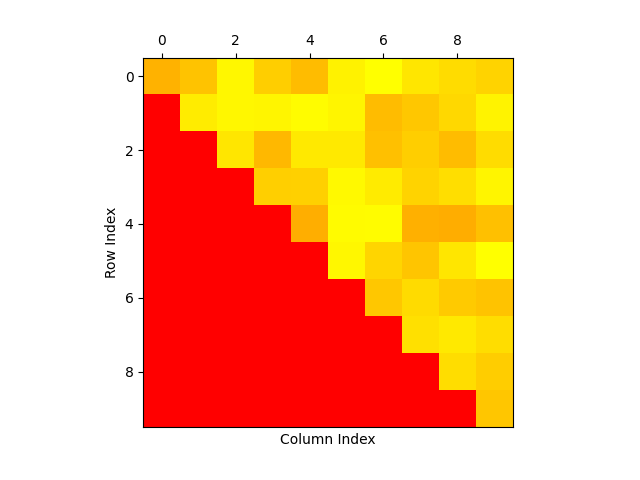
\includegraphics[scale=0.5]{tiling}
    \centering
    \caption{Tiling Representation}
    \label{fig:tiling_rep}
\end{figure}

Rather than computing the entire distance matrix in one operation, we split it into tiles. Each tile independently computes an AB-join between two segments of the input time series. This allows the computation to scale to very large input sizes and distribute the work to many independent nodes.
We finally settled on the following algorithm which is similar to the stripped down version of the SCAMP implementation. Similar to the SCAMP version, The Statistics (\(df, dg, inv\)) are computed on the Host Device and then along with the time series \(T_a, T_b\), passed on to the Device and distributed across the allocated \texttt{Resource Rectangle}. Once each PE has recieved data, then the kernel computation is triggered from the host. Each PE is only responsible to compute the aggregates for the particular tile since there are no data dependencies across tiles. The aggregates are then reduced to a Matrix Profile on the host device. This was a design decision made given the constraint on the Cerebras system for communication across PEs.

The following kernel described in Algorithm \ref{alg:tiled_algorithm} supports $t_s$ upto $835$ due to memory limitations of a PE but we experienced higher error rates at that tile size, hence we decided on a maximum $t_s$ of 830. It also supports window sizes of 3 < $m$ < \(t_s / 2\). We go deeper into the performance and limitations of a PE in Chapter \ref{chapter:measurements}.

\begin{algorithm}
    \caption{Cerebras Tiled Matrix Profiling Algorithm}
    \label{alg:tiled_algorithm}
    \hspace*{\algorithmicindent} \textbf{Input}: Time series $T_a$, $T_b$, $df$, $dg$, $inv$ and $args$ for current \textbf{Tile}.\\
    \hspace*{\algorithmicindent} \textbf{Output}: Row- and Column-Wise Aggregates for the current \textbf{Tile}
    \begin{algorithmic}[1]
        \For{$ProcessingElement \gets 0$ \textbf{to} $w * h$}
            \State $rowAggregates_{ProcessingElement} \gets (-\inf, -1);$
            \State $columnAggregates_{ProcessingElement} \gets (-\inf, -1);$
            \State $QT \gets computeQT(T_a, T_b);$
            \For{$row \gets  0$ \textbf{to} $min(args.n_x - args.exclusion\_lower, args.n_y)$}
                \For{$diag \gets args.exclusion\_lower$ \textbf{to} $min(args.n_x - args.exclusion\_upper + 1, args.n_x - row)$};
                    \State $col \gets row + diag;$
                    \State $correlation \gets QT_{diag} \cdot inv_{row} \cdot inv_{col};$
                    \State $QT_{diag} \gets QT_{diag} + df_{row} \cdot dg_{col} + df_{col} \cdot dg_{row}$
                    \If{$correlation$ $>$ $rowAggregate_{ProcessingElement, row}.value$}
                        \State $rowAggregate_{ProcessingElement, row}.value \gets (correlation, column);$
                    \EndIf
                    \If{$correlation$ $>$ $rowAggregate_{ProcessingElement, column}.value$}
                        \State $rowAggregate_{ProcessingElement, column}.value \gets (correlation, row);$
                    \EndIf
                \EndFor
            \EndFor
        \EndFor
        \State $rowAggregates \gets (-\inf, -1);$
        \State $columnAggregates \gets (-\inf, -1);$
        \For{$ProcessingElement \gets 0$ \textbf{to} $w * h$}
            \State $Merge(rowAggregates, rowAggregates_{ProcessingElement});$
            \State $Merge(columnAggregates, columnAggregate_{ProcessingElement});$
        \EndFor\\
        \Return $rowAggregates, columnAggregates;$
    \end{algorithmic}
    \label{alg:tiled_matrix}
\end{algorithm}

Algorithm \ref{alg:tiled_matrix} is the final version of the Cerebras Tiled Kernel. The core algorithm computes the aggregates for the upper half of the triangle and the other half is computed by flipping the parameters hence computing the whole tile.

The following sections of the algorithm are the primary contributors to the performance.

\begin{itemize}
    \item Compute initial $\overline{QT}$
    \item Compute pearson correlation for the current element
    \item Compute $\overline{QT}$ for the next row.
\end{itemize}

We also explored other version of tiling on the Cerebras to see if they offer any benefit in the following section.
\clearpage

\section{Tiling Options} \label{section:tiling}

The choice of tiling approaches plays a pivotal role in optimizing parallelization strategies for various computational tasks. Tiling, also known as loop blocking, partitions the computation space into smaller units, facilitating efficient data reuse and minimizing memory access overhead.
Several research studies have investigated the impact of different tiling strategies on parallel performance across diverse architectures. \cite{10}, \cite{11}

\subsection{Trapezoidal} \label{subsection:trapezoidal}

While we were looking at different tiling approaches to experiment on its impact on the performance and efficiency, we looked at Trapezoidal tiles which in theory has the same area as a square but does not allow us to elegantly handle border conditions where there are a small section or the tiles on the diagonal which contain only a upper triangle.  

\subsection{Triangles} \label{subsection:triangle}

Since we already have squares, the natural next step was to explore the implication of Triangle tiles. Although the kernel already supports triangles, The deconstruction of squares into triangles leads to more jobs to be scheduled on the Cerebras WSE. This also has an implication on the size of the \texttt{Resource Rectangle} since the number of triangles in the upper diagonal of the \textit{Distance Matrix} is more than the number of squares when deconstructed, this leads to more resource consumption but lesser execution time. This also has an impact on the memory transfer time to and from the device since a square tile and 2 triangles require the same amount of data and require reduction across two different PEs.

\section{Scheduling Approaches} \label{section:scheduling}

Given the 745,500 available PEs on the Wafer, we are limited to the size of time series we can compute in a single run. We also have a limitation on the maximum \texttt{Tile Size} that can be allocated on a single PE of 835. This creates a limitation on the size of time series we can process in one shot. Equation \ref{eq:series_decomposition} provides the number of tiles a given series of size $s$ will be decomposed into. since we have only $745,500$ PEs to work with and each can compute a tile of size 835, we arrive at a maximum time series of size $s$ = 1008940 which decomposes into $744,810$ tiles where $t_s$ = 830. Although this does not factor in the availability of Wafer Scale clusters with multiple Wafers available for execution, The Cerebras SDK at it's current stage, does not provide a simple way to integrate multiple wafers for our computation. This prompted us to solve the problem of large time series by breaking up the problem size since it is designed to be parallelizable. Real world time series data sets can go in order of billion entries \cite{8}, We explore here the different scheduling approaches to compute large scale time series data efficiently. 

\subsection{One Shot} \label{section:one-shot}

From Equation \ref{eq:series_decomposition}, We arrive at the total number of tiles that need to be computed for a given matrix of size $S$, When it is lesser than the allocatable number of PEs on the wafer/simulator, we can execute the entire Matrix Profile in a single iteration or \textit{One Shot} when the number of tiles is less than 745,500.

\begin{figure}[h!]
    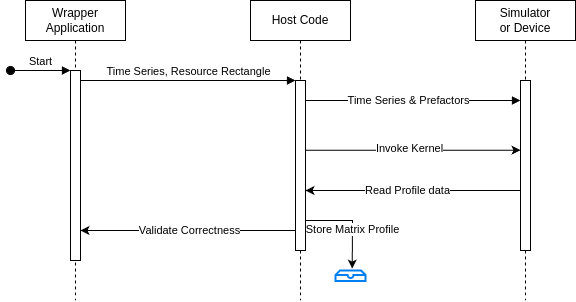
\includegraphics[scale=0.50]{job}
    \centering
    \caption{One Shot Execution of a small Time Series}
\end{figure}

The advantage of \textit{One Shot} scheduling is the reduced overhead of PE allocation and fewer memory transfer. In Practice, we found that the One Shot execution of a time series to be more demanding on the device in comparison to \textit{Iterative} execution due to the overhead of a larger \texttt{Resource Rectangle} configurations which involves larger memory transfers\footnote{We ran into errors when moving data more than 40 GB through the interface, which ran into RPC timeouts to the device. The fix for this is upcoming in the next SDK release}.

\subsection{Iterative} \label{section:iterative}

Since the algorithm allows us to execute tiles out of order, It gives us the flexibility to schedule different tiles on any PE configuration, The following approach splits the execution into smaller chunks which are then scheduled for execution in smaller \texttt{Resource Rectangles}

\begin{figure}[h!]
    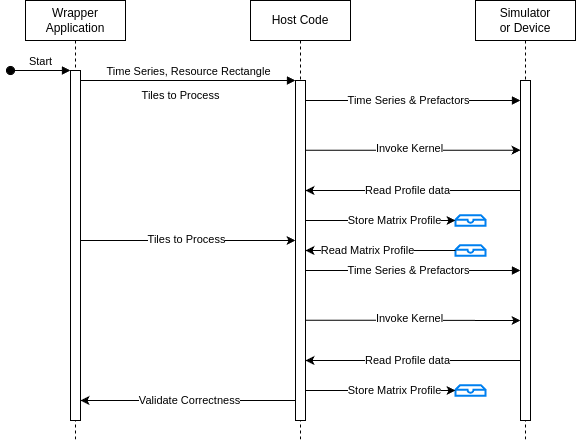
\includegraphics[scale=0.50]{iterative_job}
    \centering
    \caption{Iterative Execution of a large Time Series}
\end{figure}

When the total number of tiles is not enough to fit into a available \texttt{Resource Rectangle}, We chunk the tiles into smaller sections that are iteratively run on the Device/Simulator. This was useful to compute the Matrix Profile of very large data sets. The profile data is updated between iterations. This is possible due to the modularity of the algorithm, allowing us to split the computation into smaller steps.
